% tikz is a package that allows you to do graphics
% in a LaTeX-like style; it comes with libraries
% for all kinds of applications, including digital
% circuits
%
% the standalone class allows us to work on a
% picture independent of the main document that
% will use it; check the documentation for all
% the details
\documentclass[tikz,margin=10pt]{standalone}

\usetikzlibrary{circuits.logic.US}

\begin{document}
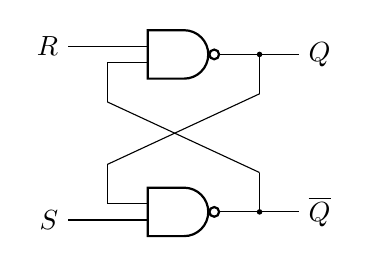
\begin{tikzpicture}[circuit logic US, every circuit symbol/.style={thick}]
  % gates
  \node[nand gate,inputs={nn},point right] (nand1) at (0,1) {};
  \node[nand gate,inputs={nn},point right] (nand2) at (0,-1) {};
  % inputs
  \draw (nand1.input 1) -- ++(left:1) node [left] {\(R\)};
  \draw (nand2.input 2) -- ++(left:1) node [left] {\(S\)};
  % outputs
  \draw (nand1.output) -- ++(right:1) node [right] {\(Q\)};
  \draw (nand2.output) -- ++(right:1) node [right] {\(\overline{Q}\)};
  % input nubs for cross coupling  
  \draw (nand1.input 2) -- ++(left:0.5) -- ++(down:0.5) coordinate (x1);
  \draw (nand2.input 1) -- ++(left:0.5) -- ++(up:0.5) coordinate (x2);
  % output nubs for cross coupling
  \draw (nand1.output) -- ++(right:0.5) coordinate (d1)
                       -- ++(down:0.5) coordinate (y1);
  \draw (nand2.output) -- ++(right:0.5) coordinate (d2)
                       -- ++(up:0.5) coordinate (y2);
  % the cross coupling!
  \draw (x1) -- (y2);
  \draw (x2) -- (y1);
  % finally draw dots for connections
  \fill (d1) circle [radius=1pt];
  \fill (d2) circle [radius=1pt];
\end{tikzpicture}
\end{document}
